% !TeX spellcheck = es_ES
\documentclass[titlepage,11pt]{article}
\usepackage[spanish,mexico]{babel}
% !TeX root = informe.tex
\usepackage{alphalph}
\makeatletter
\newcommand*{\fnsymbolsingle}[1]{%
	\ensuremath{%
		\ifcase#1%
		\or *%
		\or \dagger
		\or \ddagger
		\or \mathsection
		\or \mathparagraph
 		\or	\diamond
 		\or	\aleph
% 		\or	\backepsilon %needs amssymb or something
 		\or	\flat
		\else
		\@ctrerr
		\fi
	}%
}
 \newcommand*{\myfnsymbol}[1]{%
 	\myfnsymbolsingle{\value{#1}}%
 }

\makeatother
\newalphalph{\fnsymbolmult}[mult]{\fnsymbolsingle}{}
\renewcommand*{\thefootnote}{%
\fnsymbolmult{\value{footnote}}%
}









%\usepackage{alphalph}
%\makeatletter
% \newcommand*{\myfnsymbolsingle}[1]{%
% 	\ensuremath{%
% 		\ifcase#1% 0
% 		\or % 1
% 		*%   
% 		\or % 2
% 		\dagger
% 		\or % 3  
% 		\ddagger
% 		\or % 4   
% 		\mathsection
% 		\or % 5
% 		\mathparagraph
% 		\or
% 		\diamond
% 		\or
% 		\aleph
% 		\or
% 		\backepsilon
% 		\or
% 		\flat
% 		\else % >= 7
% 		\@ctrerr  
% 		\fi
% 	}%   
% }   
% \makeatother
% 
% \newcommand*{\myfnsymbol}[1]{%
% 	\myfnsymbolsingle{\value{#1}}%
% }
%%  remove upper boundary by multiplying the symbols if needed
%
% \newalphalph{\myfnsymbolmult}[mult]{\myfnsymbolsingle}{}
% \renewcommand*{\thefootnote}{%
% 	\myfnsymbolmult{\value{footnote}}%
% } % Footnotes lindas
\usepackage{graphicx, tikz, subcaption}

\usepackage[onehalfspacing]{setspace}

\usepackage{ieeetrantools}
% HYPERREF
\usepackage{xcolor}
\definecolor{visigrey}{rgb}{.1,.15,.15} % Color de referencias/links
\usepackage[
	allcolors=visigrey, % !todos los colores verde
	colorlinks=true, 
]{hyperref} %Hyperref antes de geometry!

\usepackage{pdfpages}
\usepackage[a4paper,left=2cm,right=2cm]{geometry}
\geometry{top=1cm,bottom=.5cm}
\savegeometry{titlepage}
\geometry{top=2cm,bottom=2cm}
\savegeometry{main}



\usepackage[T1]{fontenc}
\usepackage[utf8]{inputenc}
%\usepackage{sansmathfonts}
\usepackage{tgheros}
\renewcommand*\familydefault{\sfdefault}

\usepackage[square,numbers,sort]{natbib} % sort=en orden de aparición
\bibliographystyle{unsrtnat}

\setcounter{tocdepth}{2} % El nivel (numero) decide si se numera hasta las secciones, subsecciones o subsubsecciones
\usepackage{todonotes}


\def\Matlab{\(\textrm{\textsc{Matlab}}\)} %^\textrm{®}


%% CARATULA
%\def\courtesy{Cortesía de Satellogic.}
\def\autor{Patricio Whittingslow}
\def\tema{Monografía}
\def\titulo{Estudio de la solución\\propuesta por CE Inglis\\para agujeros en placas\\con esquinas angulosas}
\def\legajo{55423}
\def\carrera{Ingeniería Mecánica}
\def\empresa{Deformación y fractura de materiales}
\def\fecha{\today}
\def\colorborde{black} % 'white' para que no tenga borde

% GLOSARIO
\usepackage[sort=none,abbreviations]{glossaries-extra}
\setabbreviationstyle{long-short}

\newabbreviation{fem}
{FEM}
{modelo de elementos finitos}


\newglossaryentry{bias}
{
	name=Bias,
	text=bias,
	description={Refinamiento de malla controlada por el usuario para reducir error o aumentar precisión en un punto de interés.}
}

\newglossaryentry{lst}
{
	name=Linear Strain Triangle,
	text=LST,
	description={Elemento triangular de 6 nodos. Puede captar gradientes lineales de tensión con precisión arbitraria.}
}

%% DIFFERENTIAL OPERATOR
\makeatletter
\providecommand*{\diff}%
{\@ifnextchar^{\DIfF}{\DIfF^{}}}
\def\DIfF^#1{%
	\mathop{\mathrm{\mathstrut d}}%
	\nolimits^{#1}\gobblespace}
\def\gobblespace{%
	\futurelet\diffarg\opspace}
\def\opspace{%
	\let\DiffSpace\!%
	\ifx\diffarg(%
	\let\DiffSpace\relax
	\else
	\ifx\diffarg[%
	\let\DiffSpace\relax
	\else
	\ifx\diffarg\{%
	\let\DiffSpace\relax
	\fi\fi\fi\DiffSpace}

%\usepackage{bigfoot} % to allow verbatim in footnote
\usepackage[numbered,framed]{matlab-prettifier}



\let\ph\mlplaceholder % shorter macro
\lstMakeShortInline"
\renewcommand{\lstlistingname}{Código}
\renewcommand{\lstlistlistingname }{Códigos \Matlab}
\lstset{
  style              = Matlab-editor,
  basicstyle         = \mlttfamily,
  escapechar         = ",
  mlshowsectionrules = true,
  numbers = none,
  tabsize=4,
  escapeinside={`}{`},
}

\begin{document}

    \def\headingtype{\bf \small}
\loadgeometry{titlepage}
\begin{titlepage}
	\centering
	\begin{tikzpicture}[remember picture, overlay]
	\coordinate (top_right) at 
	([xshift=-2.5cm, yshift=-2.5cm]current page.north east);
	\coordinate (top_left) at 
	([xshift=2.3cm, yshift=-1.8cm]current page.north west);
	\coordinate (bottom_right) at 
	([xshift=-1.8cm, yshift=1.8cm]current page.south east);
	\node[inner sep=0, anchor=north west] at (top_left) {\href{http://www.itba.edu.ar}{
\includegraphics[height=25mm, clip]{caratula/logoitba.jpg}}};
	\node[yshift = 0.3cm, inner sep=0, anchor=north east] at (top_right) {
	\begin{tabular}{r}
	 {\headingtype \emph{\autor}} \\ [-2pt]
		{\headingtype Legajo N$^\circ$\legajo} \\[-2pt]
		{\headingtype \carrera} \\[-2pt]
		{\headingtype \emph{\empresa}} \\[-2pt]	
	\end{tabular}
	};
	\draw[double, line width = 0.5pt, color = \colorborde] (top_left) rectangle (bottom_right);
	\end{tikzpicture}\par
	\vfill
	{\Huge \bf  \tema \par}
	\vspace{2.0cm}
	{\LARGE \bf \titulo \par}
	\vspace{2.0cm}
	{\Large \fecha \par}
	\vfill
	{\centering
		
\includegraphics[width=\textwidth]{caratula/subcaratula.png}
	}
\end{titlepage}
\loadgeometry{main}



\begin{abstract}
Un resumen deberia tener menos que 250 palabras y no contener referencias.

\end{abstract}

\newpage
\tableofcontents
\newpage
\printunsrtglossaries % list all entries

\vfill
\hrule
\vspace{-1cm}
\subsection*{Nota del autor}
Si el documento es abierto desde un lector PDF moderno (Chrome, Adobe Acrobat Reader, y más), se podrá navegar el mismo mediante las referencias (haciendo click derecho).

Pueden pedir la malla usada para la resolución del FEM dirigiendosé a mi mail pwhittingslow\{at\}itba.edu.ar .
\newpage


\section{Solución de Inglis}
El dominio estudiado de Inglis \cite{inglis1913} es una placa infinita con un agujero elíptico de dimensiones $a$ y $b$ (figura \ref{fig:dom}). El espesor de la placa es mucho mayor que la dimension del agujero, por ende se puede tratar el problema con deformaciones planas (plane strain). 


\begin{figure}[htb!]
	\centering
	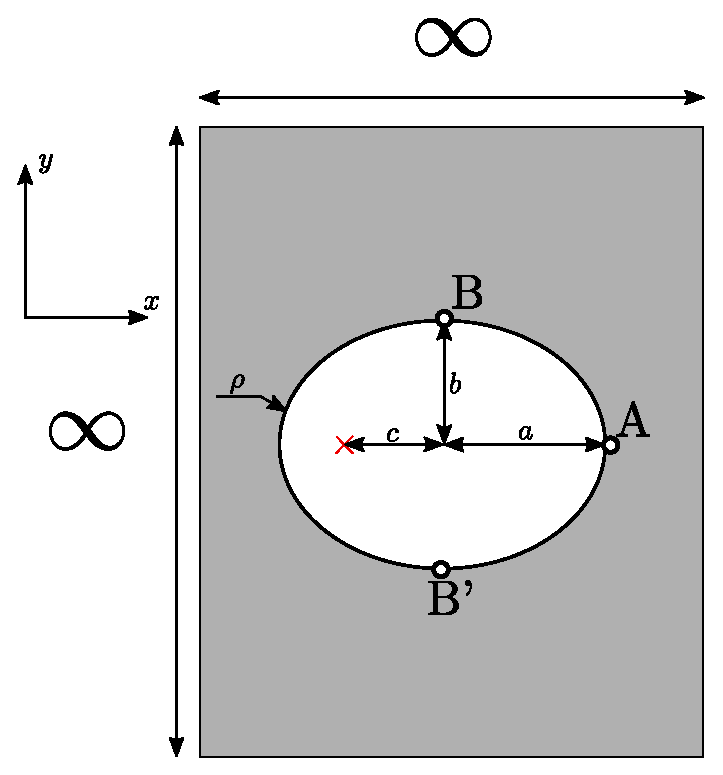
\includegraphics[width=0.5\textwidth]{fig/domain_diagram.eps}
	\caption{Dominio propuesto por Inglis con los puntos de interés $B$ y $A$.}
	\label{fig:dom}
\end{figure}

Para la resolución cómoda del dominio propuesto, Inglis trabaja en un sistema de coordenadas hiperbólicas. Se definen a continuación la parametrización de estas

\begin{IEEEeqnarray}{c}
x =c \cdot \cosh(\mu)  \cos(\nu) \label{eq:transform}\\ \nonumber
y = c \cdot \sinh(\mu)  \sin(\nu)
\end{IEEEeqnarray}
donde $c = \sqrt{|a^2-b^2|}$ es la distancia del centro hasta uno de los focos de la elipse. Cabe destacar que las iso-lineas de $\mu$ y $\nu$ son ortogonales.


\begin{figure}[htb!]
	\centering
	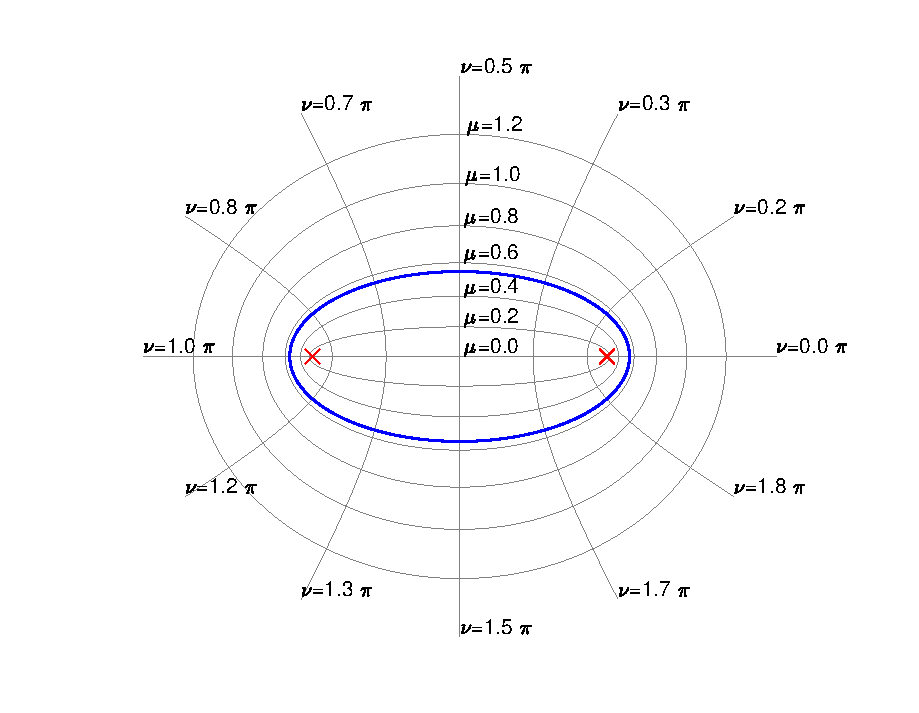
\includegraphics[width=0.8\textwidth]{fig/elliptical_coord_cut.eps}
	\caption{Coordenadas hiperbólicas (elípticas). Los focos están marcados con cruces rojas. Se dibujó en azul una elipse de relación $\frac{a}{b}=2$ que podría ser el caso de un estudio.}
	\label{fig:ellipticalCoords}
\end{figure}


Para trabajar el cálculo infinitesimal en estas coordenadas se requiere además definir dos factores de escala $h_\mu$ y $h_\nu$

\begin{IEEEeqnarray}{c}
h_\mu = h_\nu = h = c \sqrt{ \sinh^2 \mu + \sin^2 \nu}
\end{IEEEeqnarray}
Esta ecuación nos dá la longitud de los vectores base en este sistema de coordenadas. Esto significa que un diferencial de área es 
\[
\diff A = h_\mu h_\nu \diff \mu \diff \nu
\]

Inglis procede a desarrollar la teoría de elasticidad en coordenadas hiperbólicas hasta llegar a la expresión de tensiónes

\begin{IEEEeqnarray}{c}
\sigma_{\mu \mu}=\frac{E}{1+\lambda}\left[e_{\mu\mu}+\frac{\lambda}{1-2 \lambda} \Delta\right] \\
\sigma_{\nu \nu}=\frac{E}{1+\lambda}\left[e_{\nu \nu}+\frac{\lambda}{1-2 \lambda} \Delta\right] \\
\sigma_{\mu \nu}=\frac{E\cdot e_{\mu \nu}}{2(1+\lambda)}
\end{IEEEeqnarray}

\newcommand{\spartial}[2]{\frac{\partial #1}{\partial #2}}
\newcommand{\dpartial}[2]{\frac{\partial^2 #1}{\partial #2^2}}
donde $\lambda$ y $E$ son el módulo de Poisson y módulo de Young, respectivamente, del material. $e$ es la deformación y $\Delta$ es la dilatación
\begin{IEEEeqnarray}{c}
e_{\mu \mu} = \frac{1}{h} \spartial{u_\mu}{\mu} + h^2 u_\nu \spartial{h}{\nu} \\
e_{\nu \nu} = \frac{1}{h} \spartial{u_\nu}{\nu} + h^2 u_\mu \spartial{h}{\mu} \\
e_{\mu \nu} = \spartial{(u_\nu h^{-1})}{\mu} + \spartial{(u_\mu h^{-1})}{\nu}
\end{IEEEeqnarray}


\[
\Delta = \frac{1}{h^2} \left( \spartial{(h u_\mu)}{\mu} + \spartial{(h u_\nu)}{\nu} \right) 
\]
donde $u_\mu$ y $u_\nu$ son los desplazamientos en las direcciones $\mu$ y $\nu$, respectivamente. 

Resulta aparente que la solución de esta ecuación diferencial es rebuscada. Rara vez es incluida en un libro introductorio fractura de materiales. Lo que es de interés es el valor de la tensión en $A$ para el caso de tracción uniforme $\sigma$ en dirección de la hipérbola vertical $\nu=\frac{\pi}{2}$. Aquí se encuentra la tensión máxima \eqref{ec:LaEcuacion}

\begin{IEEEeqnarray}{c} \label{ec:LaEcuacion}
\sigma_{\nu\nu} = \sigma \cdot \left( 1 + 2 \frac{a}{b} \right)
\end{IEEEeqnarray}

El hallazgo de la ecuación \eqref{ec:LaEcuacion} fue de suma importancia para el desarrollo de teoría de fractura de materiales. Cuando $b$ es muy pequeño comparado a $a$ se llega al caso de una fractura. La ecuación previamente mencionada describe las tensiones halladas en materiales frágiles satisfactoriamente pero falla al momento de ser aplicada a materiales dúctiles operando cerca al rango plástico.


Una forma común de expresar la ecuación anterior es con el radio de curvatura mínimo de la elipse $\rho$. Esto permite aplicar la ecuación \eqref{ec:LaEcuacion} a fracturas de poca semejanza a una elipse. La sustitución $b=\sqrt{a\rho}$ cede la tensión en el punto $A$.

\begin{IEEEeqnarray}{c} \label{ec:TensionAradioCurv}
\sigma_{\nu\nu} = \sigma \cdot \left( 1 + 2 \sqrt{\frac{a}{\rho}} \right)
\end{IEEEeqnarray}




\clearpage
\section{Anexos}


\addcontentsline{toc}{subsection}{\listfigurename}
\listoffigures
\addcontentsline{toc}{subsection}{\refname}
\bibliography{biblio}

\end{document}